% Appendix Template

\chapter{Zielgröße} % Main appendix title

\label{AppendixE} % Change X to a consecutive letter; for referencing this appendix elsewhere, use \ref{AppendixX}

Die Zielgröße ist der reale Abstand in metern zwischen der Radaußenkante und der Innenkante der dichtesten Fahrbahnmarkierung auf Höhe des Rads, wie in folgender Skizze eingezeichnet.

\begin{figure}[h]
    \centering
    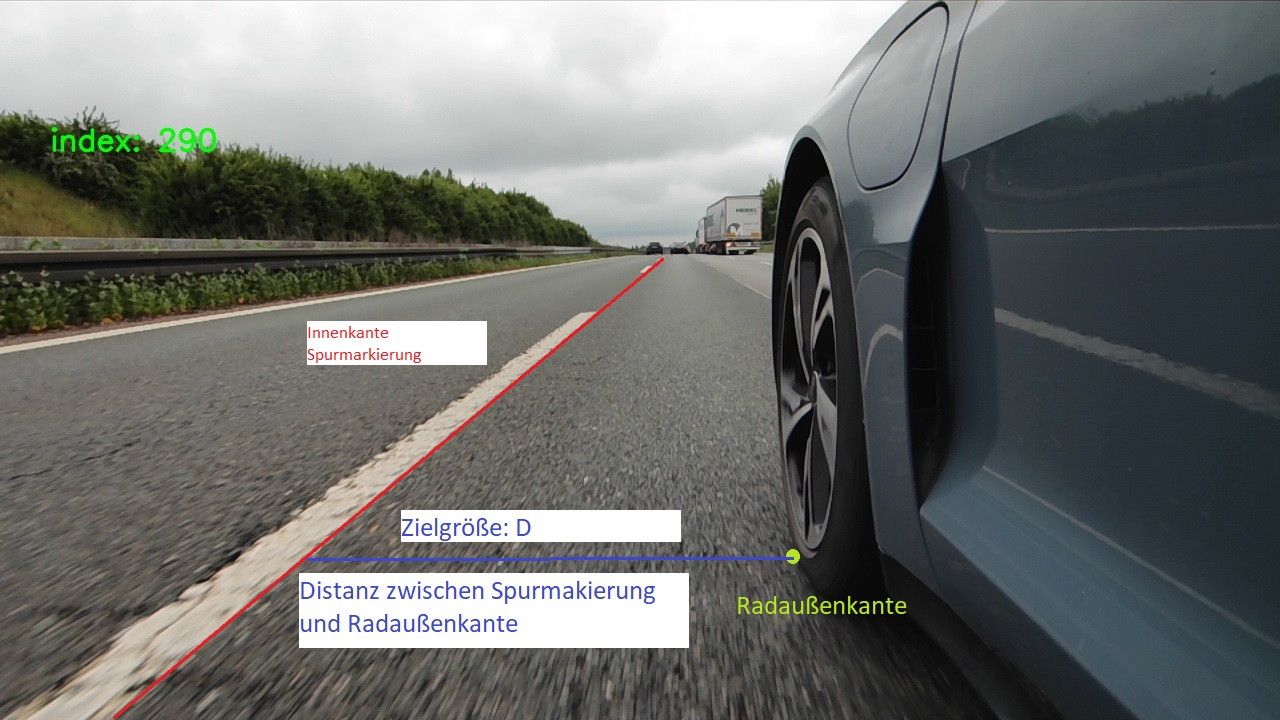
\includegraphics[width=\linewidth]{Figures/Zielgröße.jpg}
    \caption{Skizze der Zielgröße}
    \label{fig:Zielgröße}
\end{figure}